\section{Additional Experimental Results}\label{appsec:additional_exp}

In this section present the experimental results for \base\ setting which is omitted in the main paper and the details of training and each task. We use the \textsf{nanogpt}\footnote{\url{https://github.com/karpathy/nanoGPT}} codebase for language modeling.


\paragraph{Training Details.} For all settings we use $\Adam$ with $10^{-5}$ learning rate, $0$ weight decay, $\beta_1 = 0.9$, $\beta_2=0.95$, and gradient clipping with threshold equal to $1.0$. The total training budget is $10^6$ steps and we use a linear warmup in the first $2000$ steps starting from $10^{-6}$. For each step, we use a fresh sampled batch of size $64$ from population distribution. We turn off dropout and use \textsf{float16}.  We vary the depth of the transformer for different settings while the embedding size and the number of attention heads are fixed to be $512$ and $8$ respectively. 


Below we present the setting and the experimental results of each problem respectively. 

\paragraph{Modular Addition ($C_p$).} Given any positive integer $p$, the vocabulary of modular addition problem is $\{0,1,\ldots,p-1,=\}$. We generate $x=(x_1,\ldots, x_n)$ in the following way: for each $i\in[n-1]$, we independently sample $x_i$ from $\{0,1,\ldots,p-1\}$ and set $x_n$ = `='. The label is $f^*(x) = \sum_{i=1}^{n-1}x_i\mod p$ and CoT $c(x)$ is $(\sum_{i=1}^{k}x_i\mod p)_{k=1}^{n-1}$.
	Unsurprisingly, this task is an easy task for transformers because attention can easily express the average function across different positions, and so is the sum function.  Then the feedforward layers can compute the modulus of the sum and $m$. We note that the high training accuracy here is not contradictory with our \Cref{thm:AC0_upper_bound}, because our sequence length is not long enough and \textsf{float16} is like log-precision. This intuitive argument is elegantly extended to all solvable groups by leveraging Khron-Rhodes decomposition theorem by \citet{liu2022transformers}. 

%\zhiyuan{plotting instructions for Hong: 
%we don't need heatmap in this case as we only have one variable which is depth. I directly trained transformer on the distribution of mixed sequence length because the problem is so easy.
%
%For \cot, c2/c7\_\{127\}\_cot\_l\{n\_layer\}\_h8\_s512\_b64\_lr1e-05\_wd0.0\_bs?? for n\_layer in [1,2,3,4,5,6,7,8,9,10,11,12], use acc for now. 
%(I'm running more exps to fix the numbers for n\_layer <=4.
%
%For \hint, c2/c7\_\{127\}\_cot\_l\{n\_layer\}\_h8\_s512\_b64\_lr1e-05\_wd0.0\_bs?? for n\_layer in [1,2,3,4,5,6,7,8,9,10,11,12], use val/acc. 
%}


	
\paragraph{Permutation Composition ($S_p$).} Given any $p\in\mathbb{N}^+$, the vocabulary of permutation composition problem is $\{1,\ldots,p, (, ), =\}$. We pick $n = (p+2)m+1$ and generate $x=(x_1,\ldots, x_n)$ in the following way: for each $i\in[m]$, we set $x_{(p+2)(i-1)+1}$ as '(', $x_{(p+2)i}$ as ')' and independently sample a random permutation over $[p]$, $\sigma_i = (x_{(p+2)(i-1)+2},\ldots, x_{(p+2)(i-1)+p+1})$. We set $x_n $ to be '='. Different from other settings which only have the label at one position, we have $p$ labels for this setting, which is the composition of $\sigma_1\circ\ldots\circ\sigma_n$. The CoT $c(x)$ is  the partial composition from $\sigma_1$ to $\sigma_n$.

%\paragraph{Label (CoT):} \phantom{(3 4 2 5 1)(5 4 3 2 1)=}( 3 4 2 5 1) ( 1 5 2 4 3 )
%
%\paragraph{Input (CoT):} (3 4 2 5 1) (5 4 3 2 1) = ( 3 4 2 5 1) ( 1 5 2 4 3 )
%
%\zhiyuan{should I draw this? might need longer sequence}


As mentioned in \Cref{sec:main_result}, unless $\TC^0 = \NC^1$,  composition of $S_p$ cannot be computed by $\TC^0$ for any $p\ge 5$, since composition of $S_p$ implies the wording problem of $S_p$, which is $\NC^1$-complete under $\AC^0$ reductions. Since all constant-depth poly-embedding-size transformers can be simulated by $\TC^0$ circuits~(\Cref{thm:TC0_upper_bound}), shallow transformers are not able to solve the composition problem of $S_p$ for $p\ge 5$. Our experimental results in \Cref{fig:s5} matches this theoretic prediction very well. 


% \zhiyuan{plotting instructions for Hong:


% For \cot, s5\_\{length\}\_cot\_l\{n\_layer\}\_h8\_s512\_b64\_lr1e-05\_wd0.0\_bs?? for length in [6,14,30,62,126(??, if finished)], n\_layer in [1,2,3,4,5,6,7,8,9,10,11,12], use (1.4*acc-0.4) for now. (I'm running more exps to fix the numbers for n\_layer =1 or 2.

% For \hint, s5\_\{length\}\_hint\_l\{n\_layer\}\_h8\_s512\_b64\_lr1e-05\_wd0.0\_bs?? for length in range(3,39,3), n\_layer in [1,2,3,4,5,6,7,8,9,10,11,12], use 1.4*val/acc-0.4

% }
\newcommand{\sq}{\mathsf{sq}}

\paragraph{Iterated Squaring (IS).}  Iterated squaring refers to the following problem: given integers $r,n,p$, we define the iterated squaring function $f_{r,p}(n)\triangleq r^{2^n} \mod p$. It is often used as hardness assumptions in cryptography \citep{rivest1996time,lombardi2020fiat} that iterated squaring cannot be solved in $n-o(n)$ time even with polynomial parallel processors under certain technical conditions (\emph{e.g.}, $p$ is the product of two primes of a certain magnitude and there is some requirement on the order of $r$ as an element of the multiplicative group of integers modulo $p$). In other words, people conjecture there is no faster parallel algorithm than doing squaring for $n$ times.

\paragraph{Circuit Value Problem (CVP).} Circuit value problem is the computational problem of computing the output of a given Boolean circuit on a given input. It is complete for $\P$ under $\AC^0$-reductions. This means if one can solve CVP with constant-depth transformers (or any $\TC^0$ circuits), then any problem in $\P$ becomes solvable by $\TC^0$, which is widely believed to be impossible.

% In our experiment, we pick the vocabulary to be $\{0,1,\ldots,T-1,=, \text{\^{} 2}\}$ with $T=1000$. Given the length parameter $m$, we pick a random integer $n$ from $4$ to $m+3$. The input $x$ has the following format: $(r,p, \underbrace{\text{\^{} 2},\ldots,\text{\^{} 2}}_{n-3}, =)$ with $r$ being a random number from $0$ to $T-1$ and $p$ being a random prime from $0$ and $T-1$.
% We set the answer as $f^*(x)\triangleq f_{r,p}(n)$ and the chain of thought $c(x)$ is simply $(f_{r,p}(i))_{i=1}^n$. Though our construction does not exactly satisfy the technical conditions of the hardness assumption, our experiments still suggest that this iterated squaring problem is difficult for  vanilla transformers without CoT to express, but can be perfectly expressed with CoT even if depth is only 1.



% \zhiyuan{plotting instructions for Hong:
% For \cot, is1000\_\{length\}\_cot\_l\{n\_layer\}\_h8\_s512\_b64\_lr1e-05\_wd0.0\_bs?? for length in [6,14,30,62,126(??, if finished)], n\_layer in [1,2,3,6,9,12], use all\_acc

% For \hint, is1000\_\{length\}\_hint\_l\{n\_layer\}\_h8\_s512\_b64\_lr1e-05\_wd0.0\_bs?? for length in [6,14,30,62,126(??, if finished)], n\_layer in [1,2,3,6,9,12], use last\_acc
% }


%, as well as more experiment  details.
%\begin{figure}[H]\label{fig:base2}
%% 
%\begin{center}
%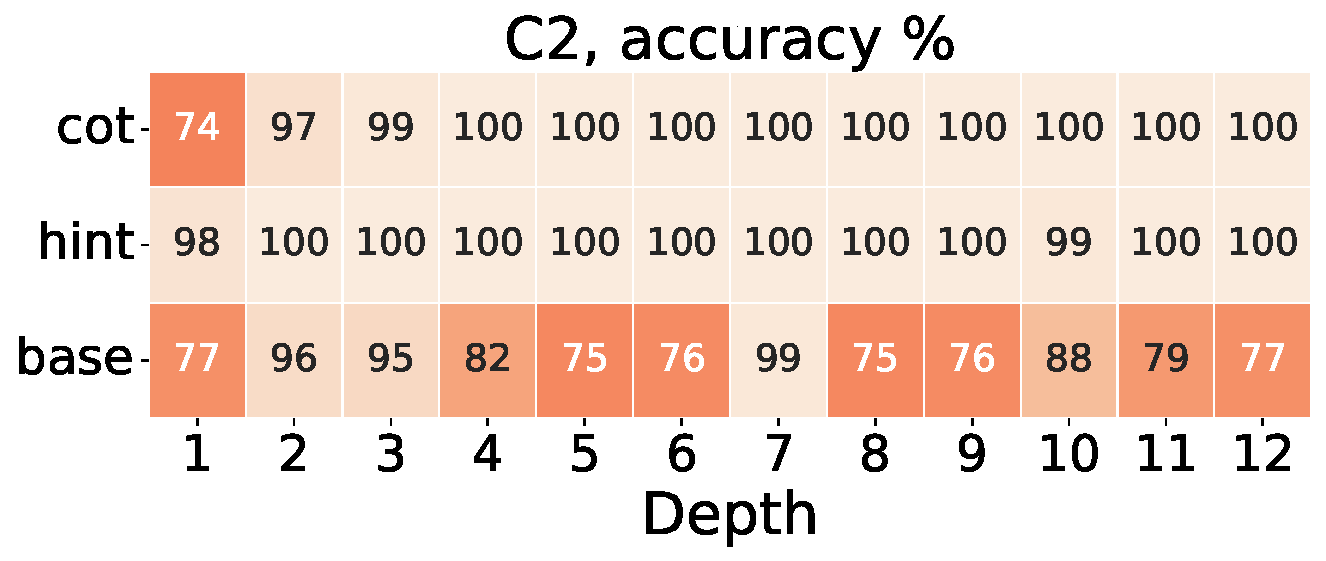
\includegraphics[width=0.46\textwidth]{figures/c2_base.pdf}
%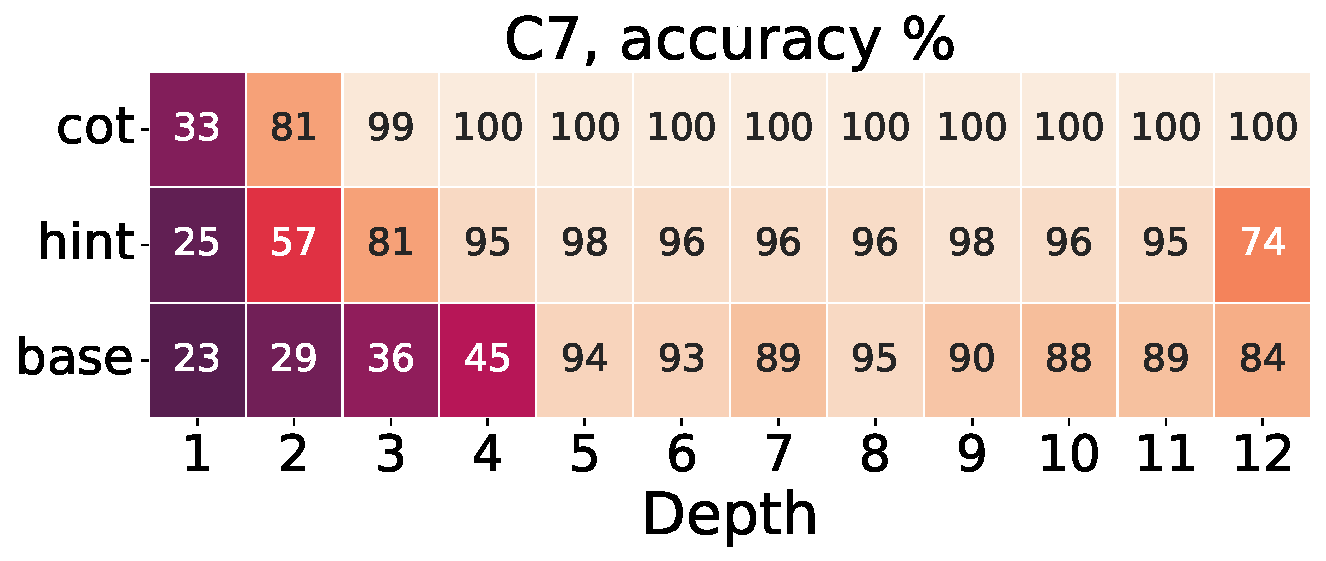
\includegraphics[width=0.46\textwidth]{figures/c7_base.pdf}
%\caption{\small Results of \base~on Modular Addition.}
%\end{center}
% 
%\end{figure}

\begin{figure}[H]
% 
\begin{center}
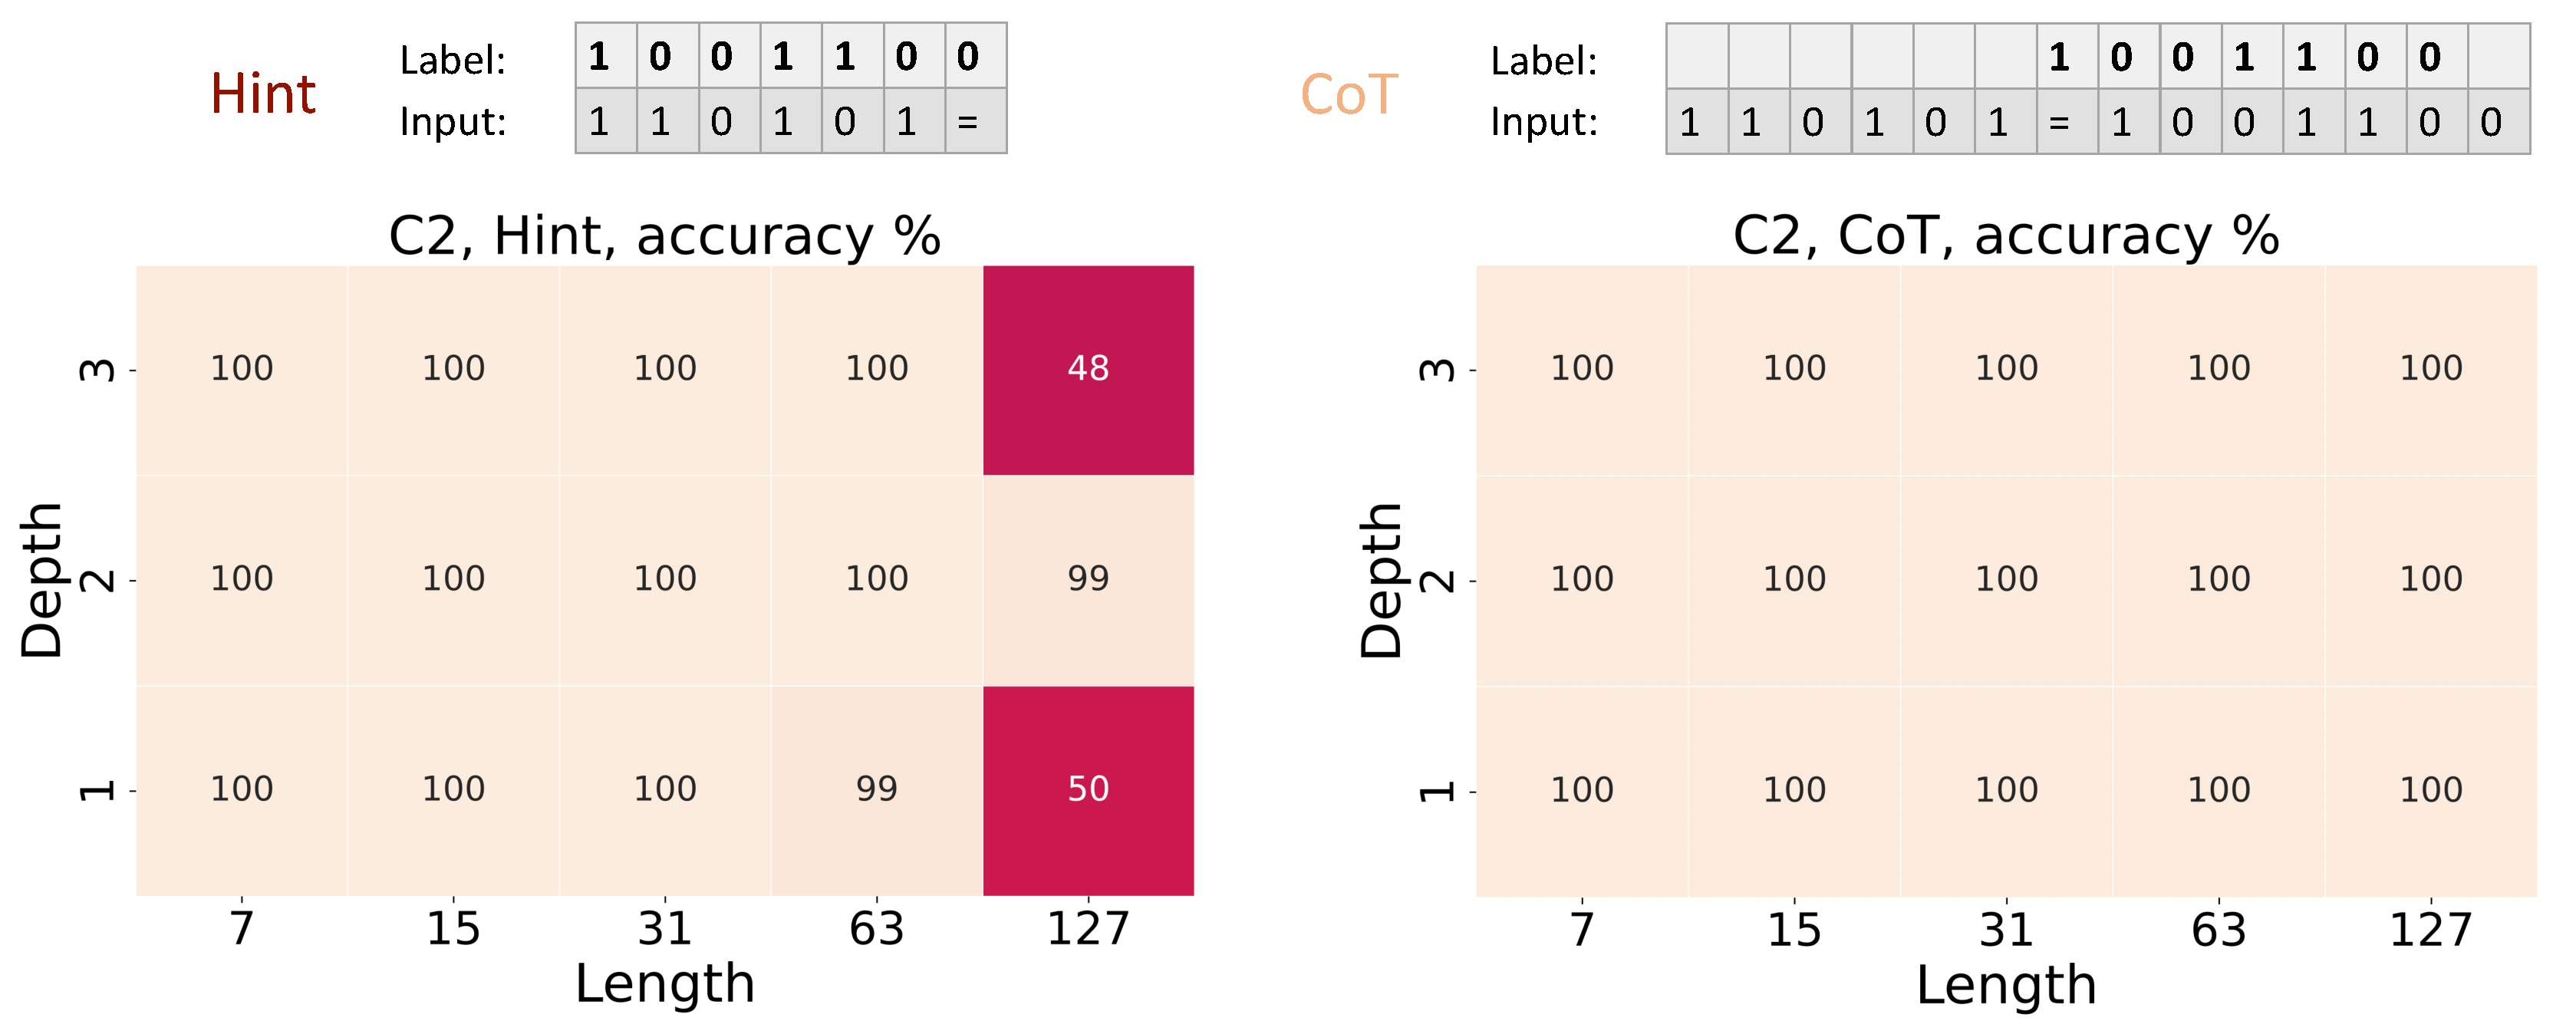
\includegraphics[width=\textwidth]{figures/c2_iclr.pdf}
\caption{Results of Modular Addition $C_2$.}\label{fig:c2}
\end{center}
\end{figure}


 \begin{figure}[H]\label{fig:base1}
% 
\begin{center}
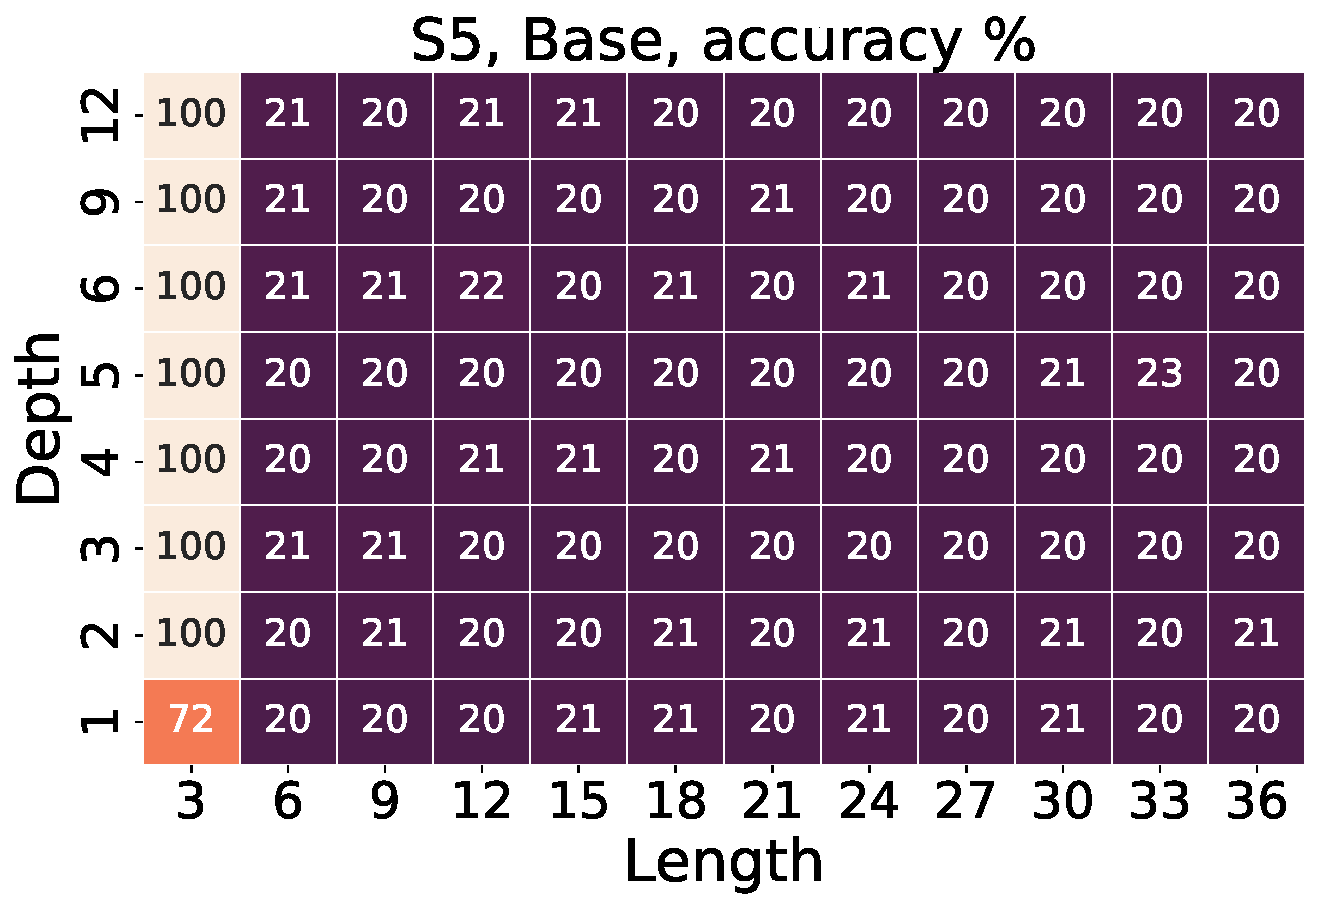
\includegraphics[width=0.328\textwidth]{figures/s5_base.pdf}
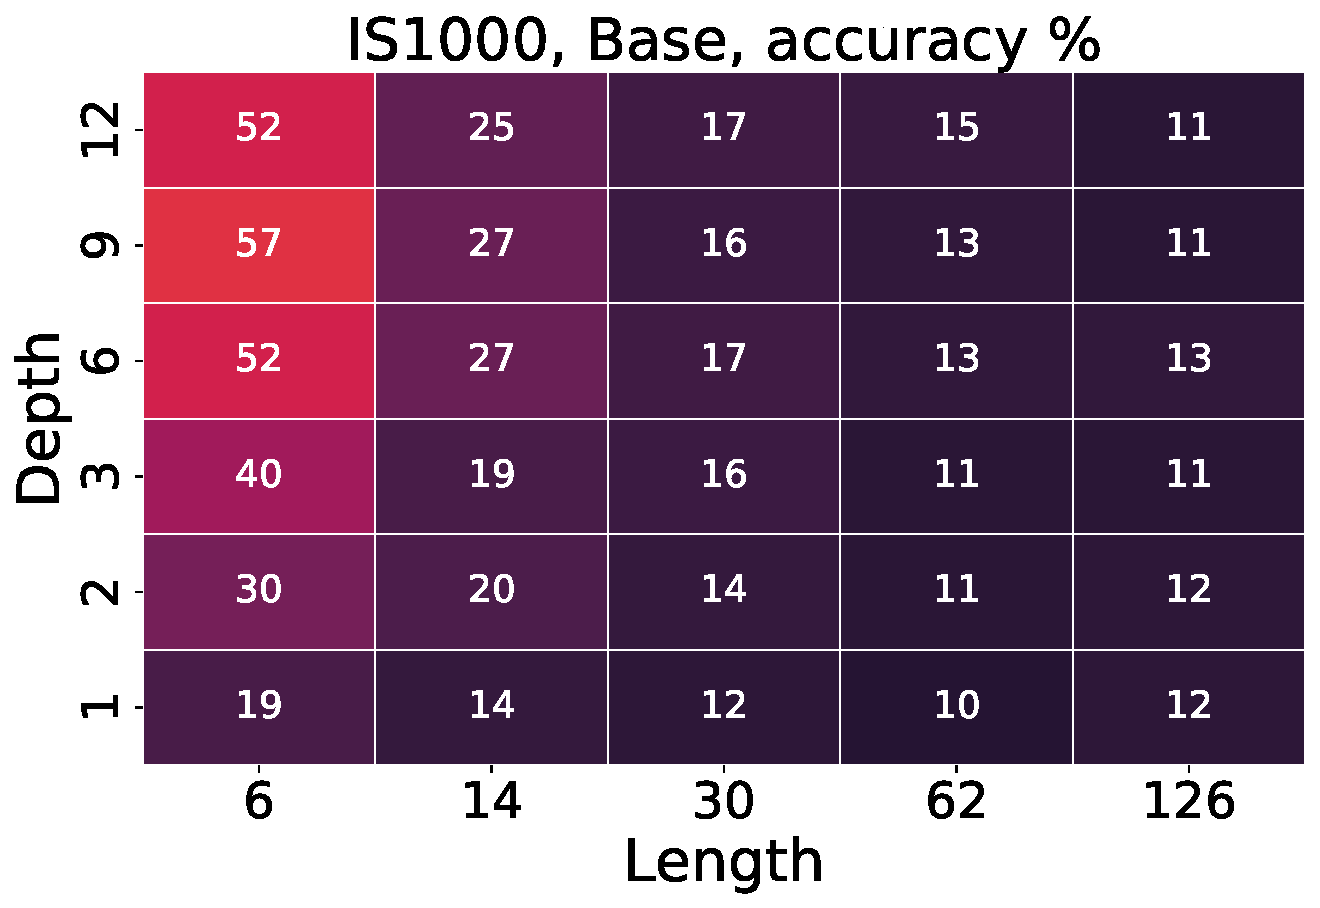
\includegraphics[width=0.328\textwidth]{figures/is1000_base.pdf}
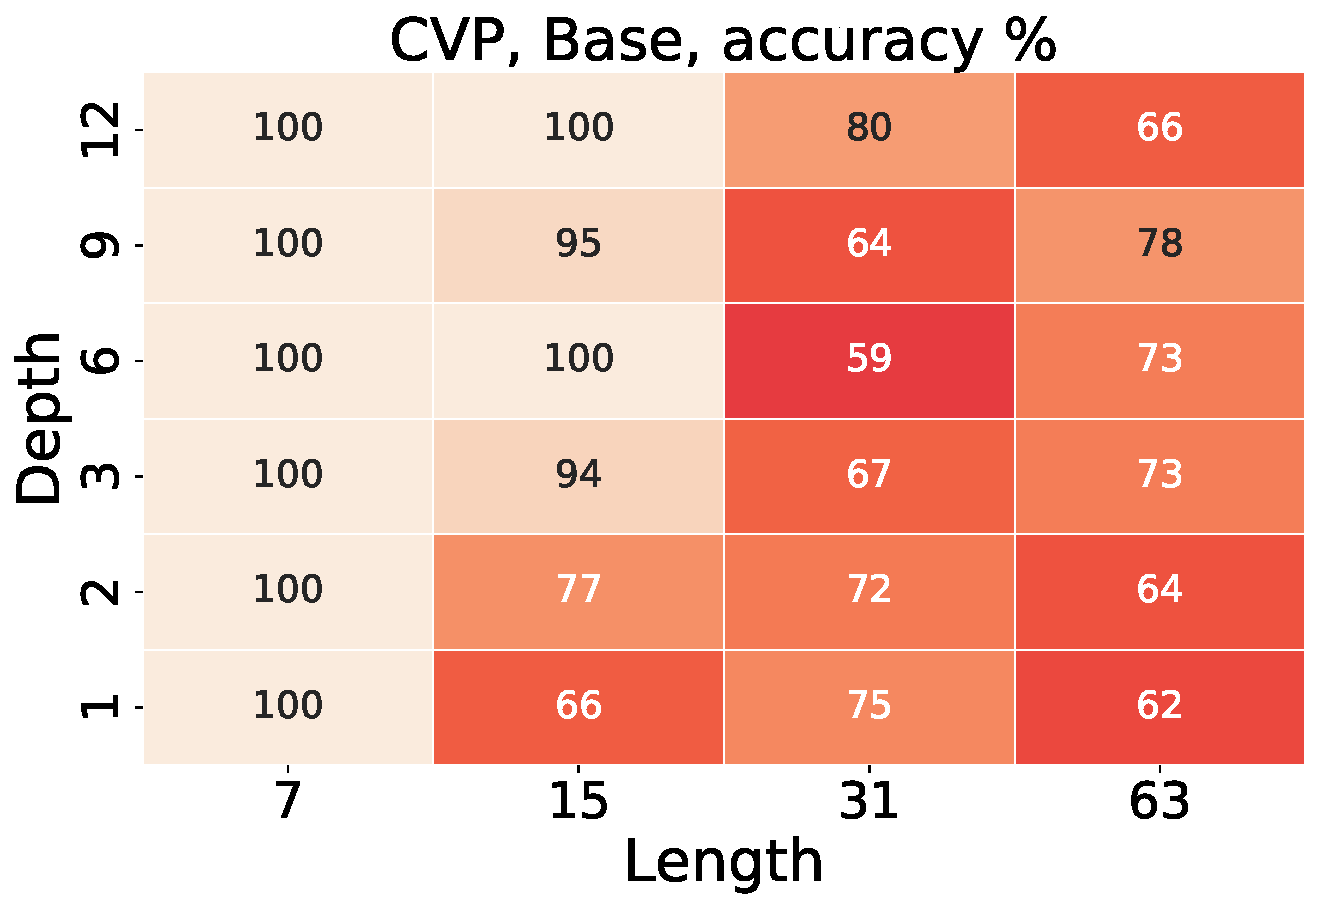
\includegraphics[width=0.328\textwidth]{figures/cvpv3_base.pdf}
\caption{Results of \base~on Permutation Composition, Iterated Squaring, and Circuit Value Problem.}
\end{center}
\end{figure}


 \begin{figure}[H]\label{fig:base2}
% 
\begin{center}
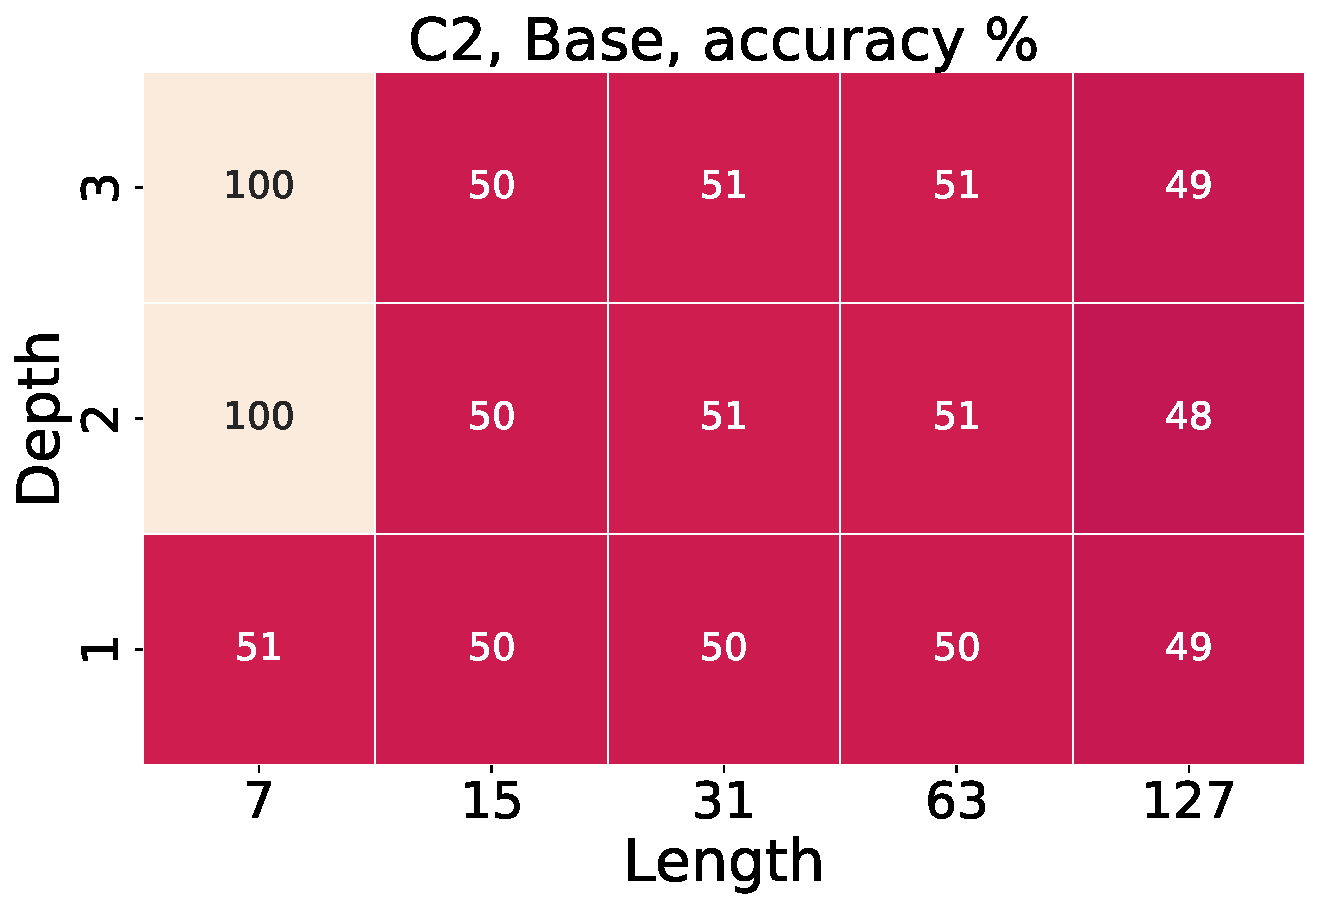
\includegraphics[width=0.49\textwidth]{figures/c2_base_val_iclr.pdf}
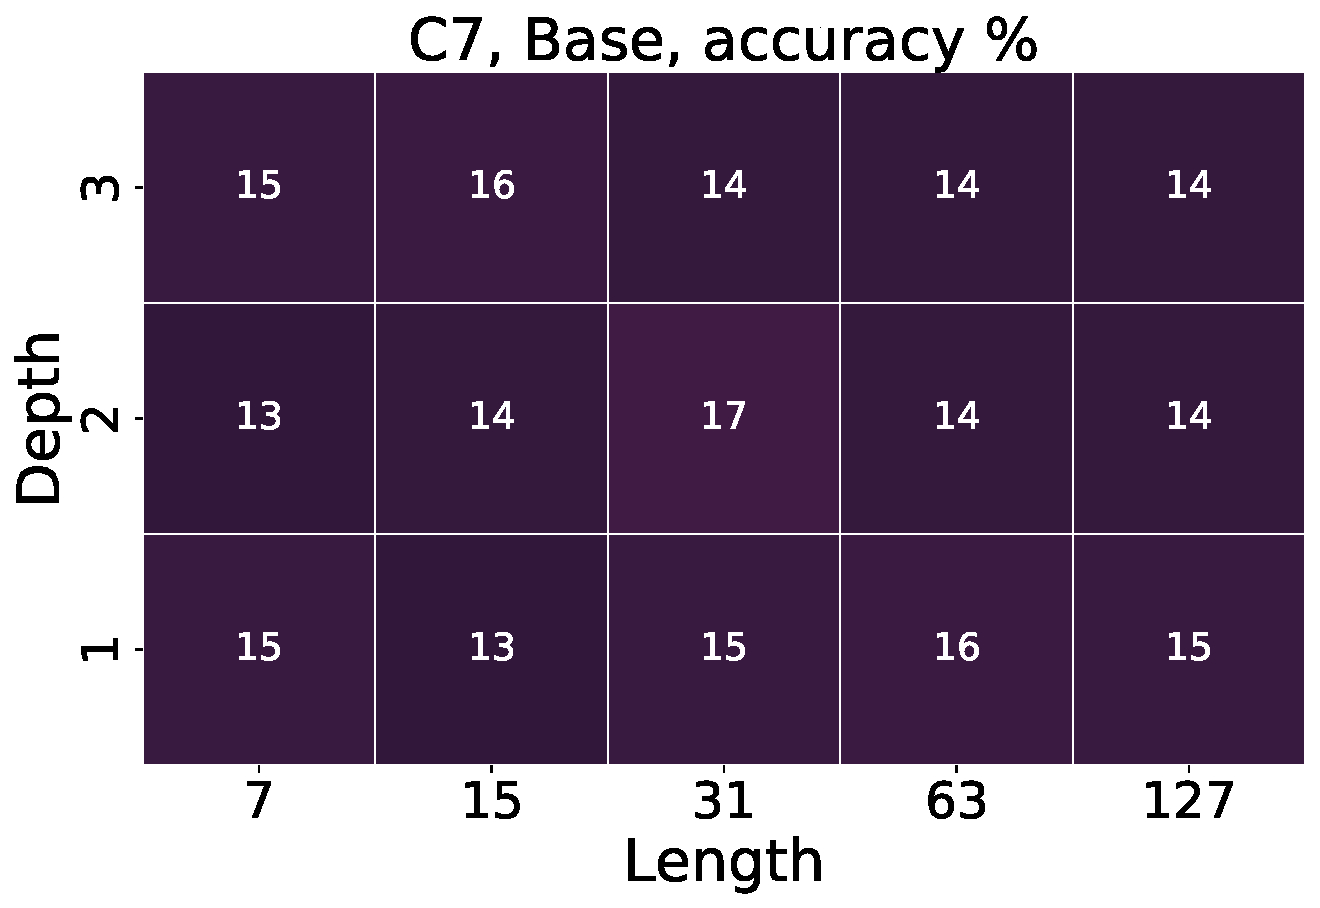
\includegraphics[width=0.49\textwidth]{figures/c7_base_val_iclr.pdf}
\caption{ Results of Modular Addition \base~on $C_2$ and $C_7$.}
\end{center}
\end{figure}


We can observe that the accuracy of \base\ setting is also lower than that of \hint\ setting.

